\chapter{Conclusion}
\label{conclusion:chapter}

This thesis has presented a study of self-organisation in peer production, a story of how hundreds of thousands of Drupalistas have organised themselves during the past fifteen years, from which three main contributions resulted. Firstly, questioning and studying the notion of contribution in CBPP communities. Secondly, identifying the general dynamics of formalisation in the organisational processes and decentralisation in decision-making, providing an in-depth account of how they are intertwined. Thirdly, offering an in-depth account of how the organisational changes explored, as shaped by the aforementioned dynamics, resulted in the emergence of a \textit{polycentric} model of governance, in which different forms of organisation, varying in their degree of \textit{organicity}, co-exist and influence each other. These insights, which fall within the field of Science and Technology Studies, contribute to the literature on Commons-Based Peer Production and Free/Libre Open Source Software, whilst also providing implications which are of interest for the practitioners in these communities.

This chapter concludes this thesis, firstly by summarising the key insights and contributions of this study to the aforementioned fields in section \ref{sec:conc:findings}, subsequently presenting a set of implications for practitioners in section \ref{sec:conc:implications}, and finally discussing possible avenues for future research in section \ref{sec:conc:future-work}.

\section{Key insights}
\label{sec:conc:findings}

This study of self-organisation in Commons-Based Peer Production was based on a single and in-depth case study which, as discussed in section \ref{sec:growth-community}, should be understood as an extreme case because of the significant growth experienced by the Drupal community. Studies focussed on a single, in-depth and extreme case are valuable to shed light on organisational aspects which are pivotal for the main body of work on Commons-Based Peer Production and Free/Libre Open Source Software. These approaches help to tackle issues derived from other research designs, such as over-generalisation, over-simplification and neglect of complexity. As discussed in chapter \ref{chapter:introduction}, previous research on self-organisation of CBPP and FLOSS communities was criticised \parencite{viegas2007hidden, mateos2008institutions} for lacking social and institutional aspects, which resulted in offering oversimplified accounts. Thus, it is through the study of extreme cases, such as this, by which it is possible to unveil these aspects of peer production, which are less prominent in smaller and organisationally simpler communities. 

\subsection{``Talk is silver, code is gold"? Beyond ``object-centric" notions of contribution in peer production}

This study shows the need to broaden our understanding of the notion of contribution in the study of peer production beyond the most traditional ``object-centric" conceptions, which in the concrete case of Free/Libre Open Source Software studies has been more prominently present in the form of ``code-centrism". The notion of contribution should be understood as a set of meanings which are under constant negotiation between the participants in peer production communities according to their internal logics of value.

This constructivist approach towards the notion of contribution has implications for studies aiming to further our understanding of Commons-Based Peer Production. For example, to show the relevance of intangible assets in these communities, such as those which emerged from this case study in the form of affective labour \parencite{hardt1999affective}. ``Object-centrism" within the notion of contribution is still commonly present in the studies of CBPP communities. For example, studies on contribution in Wikipedia are commonly focussed on the edition of articles \parencite[e.g.][]{kittur2007power, 6480229, Matei2015178}; or studies on contribution in OpenStreetMap on the edition of maps \parencite[e.g.][]{doi:10.1179/000870410X12911304958827, ijgi1020146}. While \textcite{coleman2013coding} showed a relationship --- highlighting some of these affective, moral, economic, and political dimensions --- between face-to-face events and the public in FLOSS communities, this study is novel in showing how these ``community-oriented" activities are understood as relevant contributions. This study connects a constructivist approach towards the notion of contribution to the wider literature on Commons-Based Peer Production through the concept of affective labour. Furthermore, this study provides evidence of the role which these less visible contributions play to transform the emotional experiences of the participants in becoming ``commoners", as well as to scale up the overall sense of community.

This notion of contribution also has implications for the provision of indicators that measure, aggregate and incorporate these forms of value in the technical artefacts employed to support the organisation of peer production. Hence, this finding is also relevant for more technical fields, such as Computer Science, as well as research initiatives \parencite[e.g.][]{CAPS:2017:Online} aiming to develop platforms to support and foster the development of peer production. For example, by assuming a constructivist approach, a high degree of flexibility is expected for the design of mechanisms that indicate the notion of value in the collaboration platforms employed by these communities. In other words, rather than creating tools which impose ``one-fits-all" indicators, such as ``likes", a broader understanding of contribution in peer production implies for these platforms the need to offer mechanisms that enable communities to define these indicators dynamically, allowing them to reflect the results of their processes of constant negotiation.

\subsection{Formalisation and decentralisation in peer production}

The research identified two general organisational dynamics affecting this case of a large and global Commons-Based Peer Production community as it grew over time: the formalisation of organisational processes and the decentralisation of decision-making. The exploration of the organisational processes of this case study provided a detailed account of how these dynamics are intertwined and how they shaped the overall resulting system of peer production. This is despite the main medium of the peer production activities studied being online/offline or the significant differences with regard to their main focus of action --- writing source code or organising events.

At first glance, this could be perceived as contrasting with some of the hacker values which were initially introduced in this study (see section \ref{subsec:hacker}). For example, \textcite[34-35]{levy1984hackers} explains how one of the main hacker values consists of a mistrust of authority by promoting decentralisation. Hackers avoid formal and bureaucratised systems, since these systems invoke arbitrary rules to consolidate power and react interpreting their creative impulses as a threat. However, previous chapters show how the evolution towards an increased formalisation of self-organisational processes around decision-making is explained as a means to achieve this decentralisation. These apparently contrasting ideas, which were conceptualised as a systemic contradiction from an Activity Theory perspective (see section \ref{subsec:3at}), were employed in this study as  a ``window of opportunity" (see section \ref{sec:do-ocracy}) to follow and collect data to explore the emergence of the processes and structures which the Drupal community has created over time. Formalisation and decentralisation, it was shown, resulted in the emergence of several socio-technical systems of contribution, some of which were explored in this thesis.

This finding is congruent with recent quantitative studies in FLOSS \parencite[e.g.][]{schweik2013preliminary} and CBPP communities \parencite[e.g.][]{wang2016institutional}. For example, drawing on Social Network Analysis techniques, \textcite[4]{wang2016institutional} concluded that:

\begin{quotation}
``[...] despite recent  claims  about  the value  of  loosely coordinated entrepreneurial  online  action,  the  introduction of  some structure  to  peer production  can  be  beneficial. Specifically,  providing  participants  with  the  tools  to self-organize  (e.g.,  by defining  roles  in  subprojects)  can lead  to  less  centralized  engagement; on the other hand, providing no such tools could result in participant engagement that coalesces around community leaders who exert a disproportional influence on the output of the community."
\end{quotation}

While quantitative approaches, such as \textcite{wang2016institutional}, show the generalisability of this argument, the qualitative approach followed in this study provides an in-depth account of how formalisation and decentralisation occur in peer production. In other words, this study shows how the explored self-organisational processes increased in their degree of formality over time and their relationship with the dynamic of decentralisation of decision-making. This was a limitation acknowledged by \textcite[18]{wang2016institutional} in their study because of the quantitative approach followed. It is important to consider, however, that this study was framed, as shown in the main research question, as that of a large and global CBPP community. CBPP communities may not commonly experience such an intense increase in participation, hence, it would be suggested that they commonly possess an organisational configuration which resembles that of this case study during its initial stages: characterised by having a high degree of \textit{organicity} in self-organisational processes. Nevertheless, this does not reduce the relevance of this finding, since CBPP communities growing in participation may experience similar organisational changes and be shaped by analogous dynamics, as similar empirical studies \parencite{viegas2007hidden, forte2009decentralization} suggest. Thus, this study contributes to the literature by providing an in-depth account of how these dynamics are intertwined, explaining the emergence of these different socio-technical systems of contribution, as well as how these sophisticated organisational processes work in practice. This contribution, hence, furthers our understanding of the inner workings of large and global CBPP communities in congruence with the results from the aforementioned recent quantitative studies \parencite{schweik2013preliminary, wang2016institutional}, which suggest the robustness of this finding.

\subsection{Emergence of \textit{polycentric} governance and organisational forms with different degrees of \textit{organicity}}

By bringing together empirical data from the exploration of the self-organisational processes of the case study with literature from organisational theory, this study shows the simultaneous co-existence of different forms of organisation found in a large and global case of a Commons-Based Peer Production community. These different forms vary in their degree of \textit{organicity}, which, in the case of Drupal, materialised through the emergence of different socio-technical systems of contribution. These socio-technical systems, it was shown, entail a set of interacting parts. They include people, institutions, software, hardware, procedures or rules among others. In other words, these socio-technical systems of contribution constitute complex wholes that revolve around networks of human activity systems towards a shared focus of action, in what is perceived as a contribution according to the internal logics of value of the community. Furthermore, this study provides evidence of how \textit{polycentric} governance emerged. Participants distributed authority and power over several centres of governance with coordination amongst them as part of a process of continuous negotiation, leading to the emergence of an organisational system for peer production in which different forms of organisation, varying in their degree of \textit{organicity}, co-exist.

Following a dynamic approach which highlighted and explored changes in self-organisation, the account of the emergence of \textit{polycentric} governance and organisational forms with different degrees of \textit{organicity} presented in this study, thus, contributes to continue the unveiling of the \textit{hidden order} \parencite{viegas2007hidden} of Commons-Based Peer Production communities. This account furthers our knowledge of organisation in peer production in a field which, as a result of approaching a novel phenomenon, is in an incipient state of research and in which the literature focussed on its self-organisational aspects is still scarce. This scarcity finds its exception in \citeauthor{forte2009decentralization}'s (\citeyear{forte2009decentralization}) study, whose exploration of self-organisation in Wikipedia can indeed be interpreted as depicting a simultaneous co-existence of organic socio-technical systems of contribution, in the form of Wikiprojects, with mechanistic systems with respect to the different articles produced by the participants of the well-known collaboratively built encyclopedia. Comparative studies with a wider range of case studies, especially including lesser known projects than Wikipedia and also beyond FLOSS, could confirm the generalisability of this co-existence of different forms of organisation in CBPP communities, as well as whether they also influence each other in similar ways as those found for this case study. Nevertheless, this does not undermine the relevance of this contribution, since it is through the study of extreme cases, such as Drupal, that certain organisational aspects of peer production, which are less visible in smaller and organisationally simpler communities, can be unveiled.

\section{Impact and implications of this thesis for practitioners}
\label{sec:conc:implications}

Throughout the course of this research a significant effort was carried out to disseminate the key insights presented in the previous section beyond academic environments. These insights have aroused the interest of practitioners of CBPP communities and public institutions interested in fostering peer production. As discussed in section \ref{sec:levels-organicity}, for example, the study of the notion of contribution presented in this thesis fostered a discussion within the Drupal community regarding the need to provide more visibility and acknowledgement to ``community-oriented"  contribution activities \parencite[e.g.][]{impact-contrib01:Online, impact-contrib02:Online, impact-contrib03:Online, impact-contrib04:Online, impact-contrib05:Online, impact-contrib06:Online, impact-contrib07:Online, impact-contrib08:Online, impact-contrib10:Online}. At the time of writing (September 2017) the discussion remains ongoing in an issue \parencite{impact-contrib10:Online} at Drupal.org opened by a member of the Drupal Association, in which the community is discussing and trying to envision ways to improve the visibility of these ``community-oriented" forms of contribution in the main artefacts employed for collaboration in the community, such as user profiles at Drupal.org. Through this issue the community is tackling questions such as: ``Are all the contributions equal?", ``How can we \textit{give weight} to the value of different contributions?", ``How can we track `community-oriented' contributions, such as organising a DrupalCamp?" or ``Should we consider only the recent contributions, or the whole history of them?". Figure \ref{user-contribs} below provides an illustration of the context of this discussion, in the form of a tentative proposal to assign points to different contribution activities.

\begin{figure}[H]
    \centering
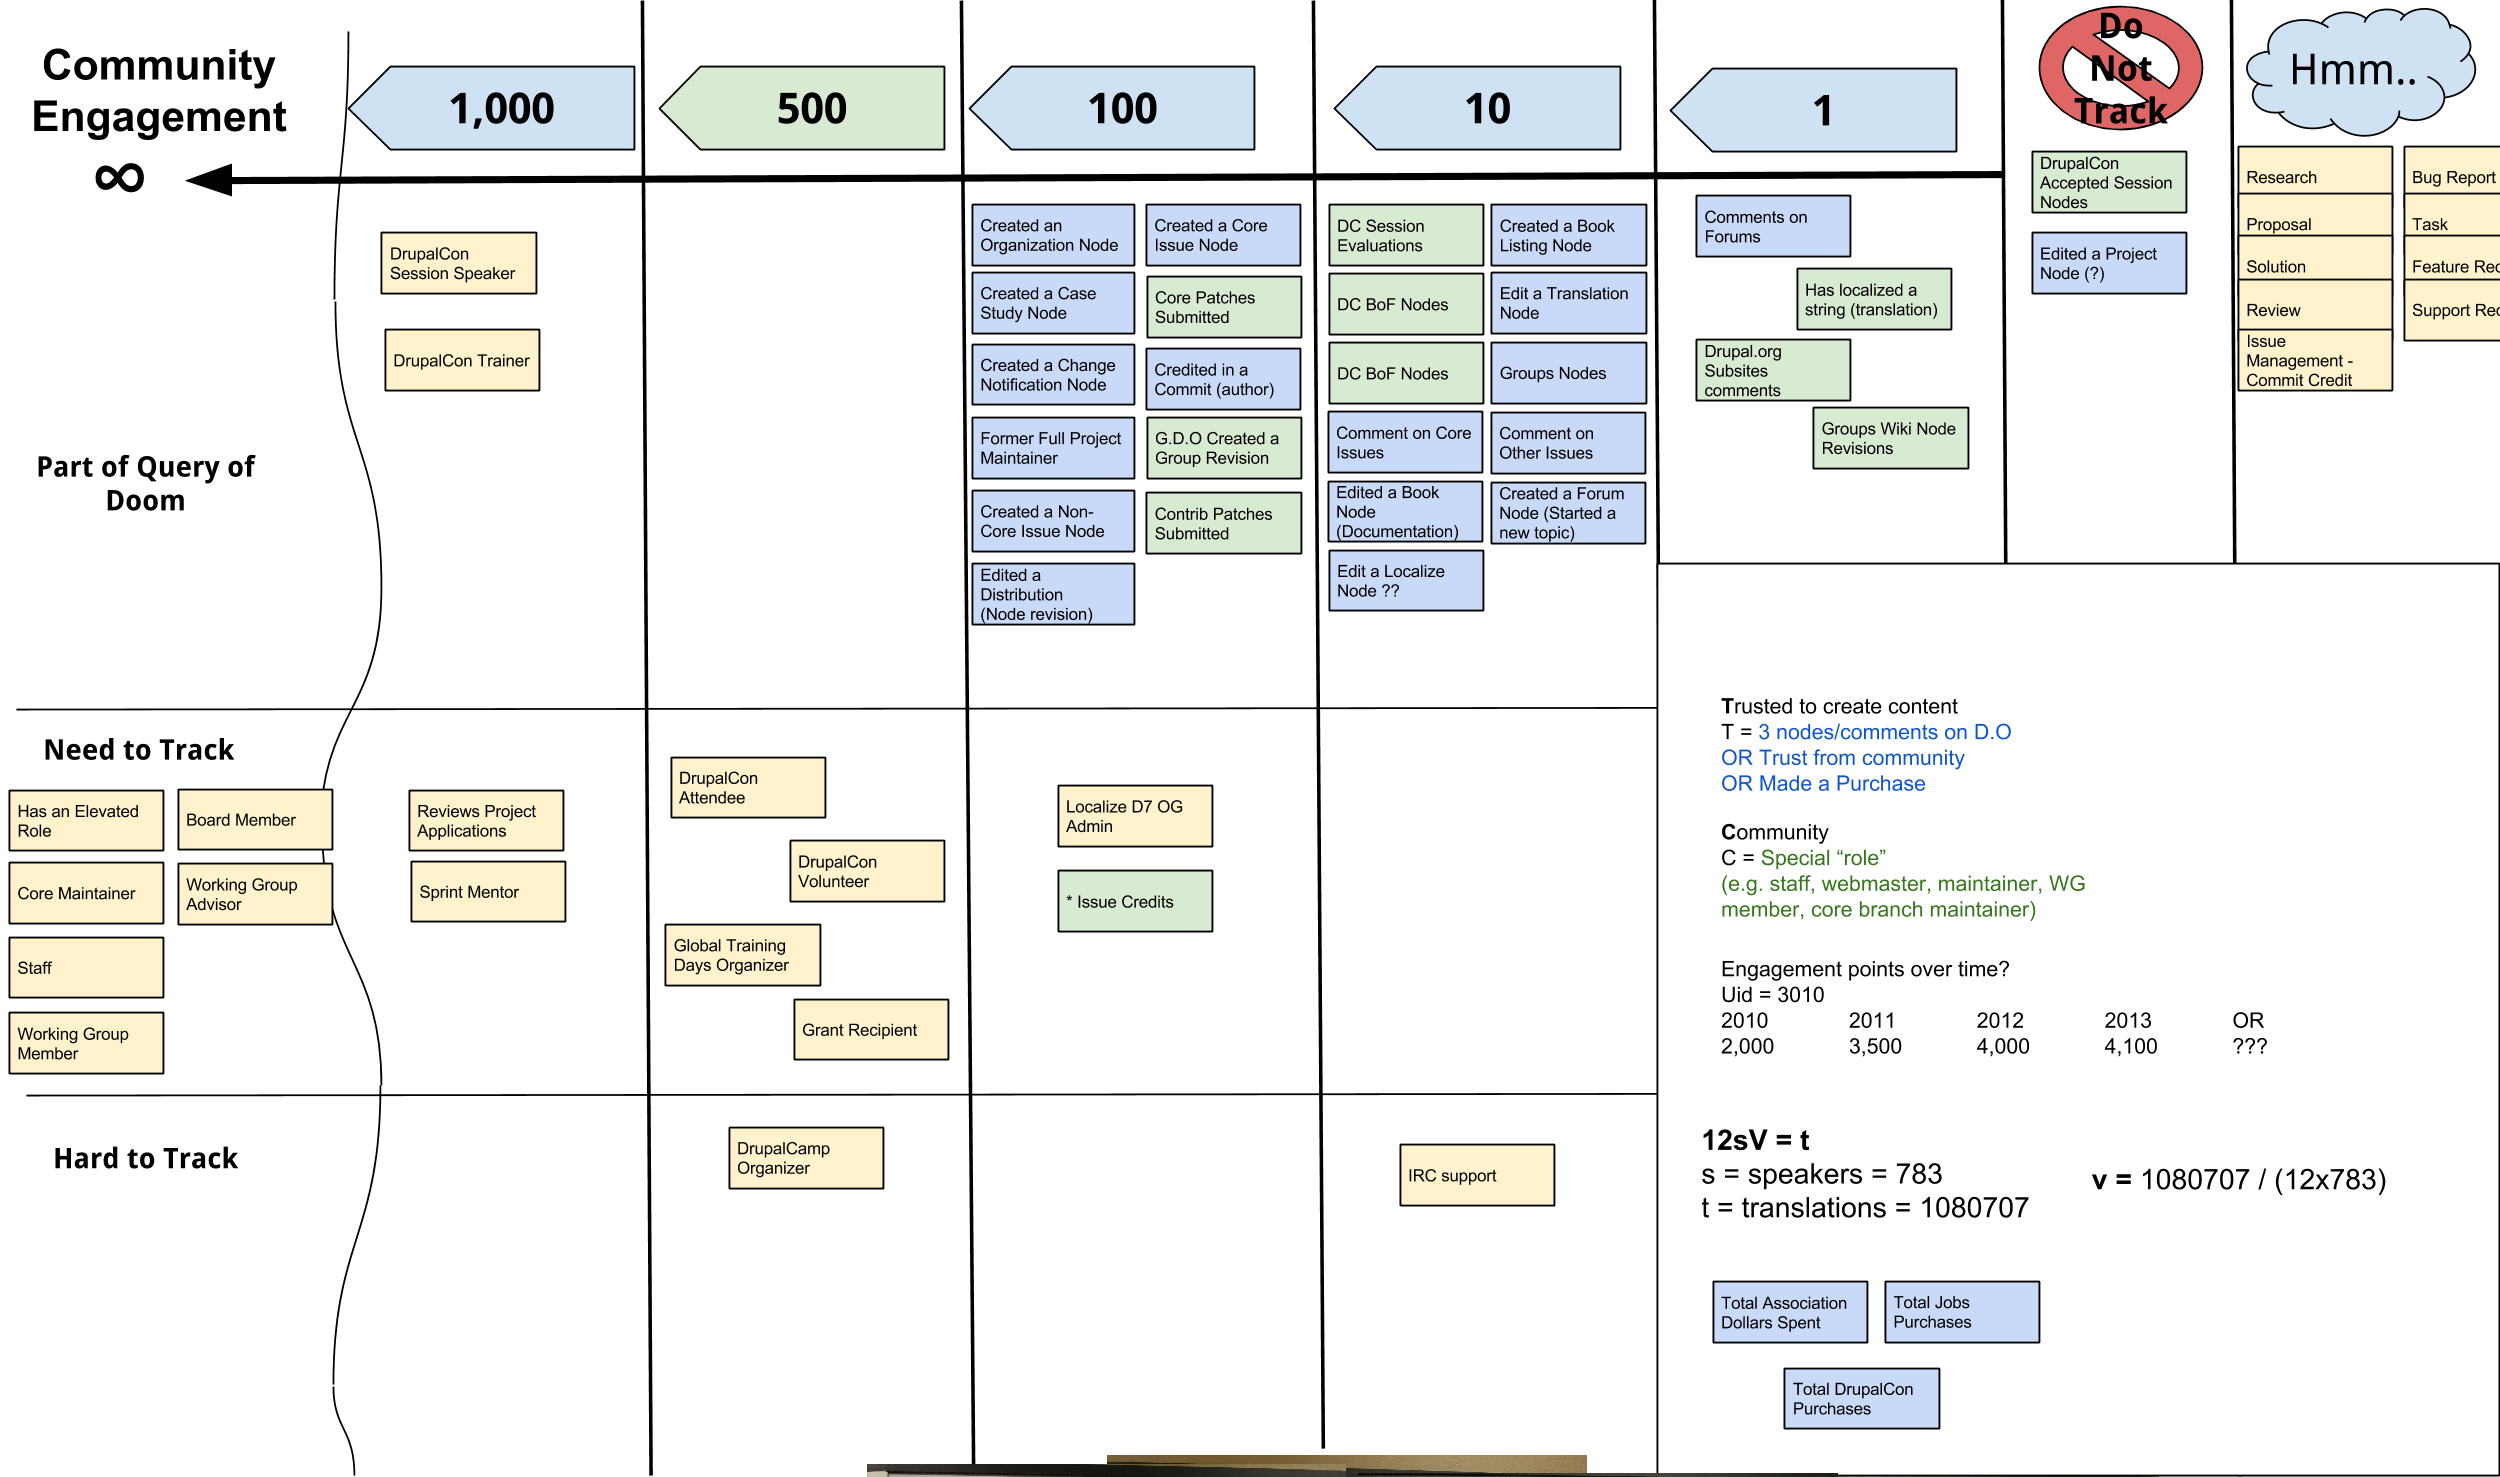
\includegraphics[width=\textwidth]{img/polycentric/contrib-cc.png}
    \caption[Artefact employed to discuss the notion of contribution in the Drupal community]%
    {Example of one of the artefacts employed to discuss the notion of contribution in the Drupal community. Picture retrieved \nth{23} September 2016, from \url{https://www.drupal.org/node/2649100}.}
    \label{user-contribs}
\end{figure}

Another example of the impact of this research in environments beyond academia is my recent participation \parencite{decidim-bcn:2017:Online} as an invited speaker by the council of Barcelona. In this event, I presented the insights related to the emergence of \textit{polycentric} governance and simultaneous co-existing forms of organisation in peer production that resulted from this case study. These insights were discussed in the context of a series of events focussed on the study of governance of digital platforms. These events are intended to develop more direct and democratic approaches for the participation of citizens in the decision-making of municipal institutions\footnote{See, for instance, \url{https://www.decidim.barcelona/} (only available in Catalan or Spanish) and \url{https://decide.madrid.es/?locale=en} to find examples of these initiatives in Barcelona and Madrid respectively.}, such as participatory budgeting.

\begin{figure}[H]
    \centering
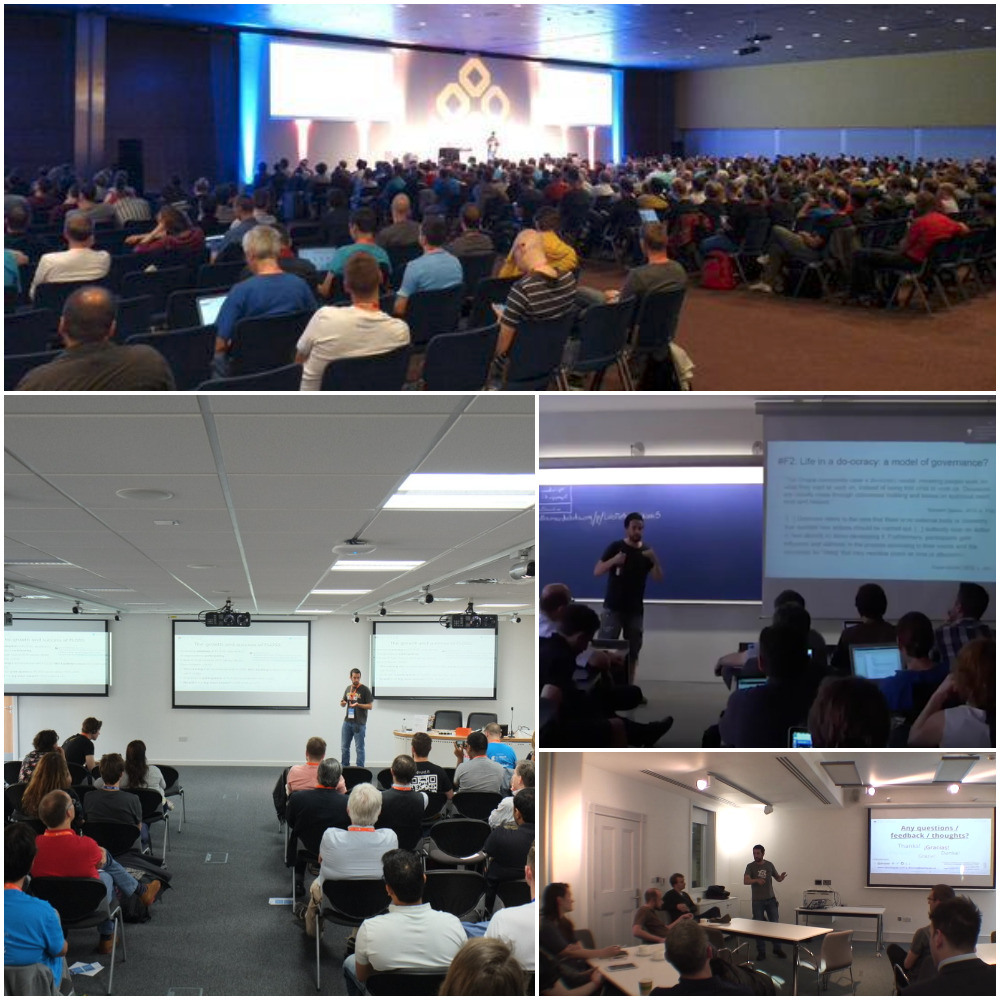
\includegraphics[scale=0.35]{img/events/drozas_events_several.jpg}
    \caption[Pictures taken during the presentation of the findings of this research in several events]%
    {Pictures taken during the presentation of the findings of this research in several events\protect\footnotemark organised by peer production practitioners and public institutions willing to foster peer production.}
    \label{drozas_events}
\end{figure}


\footnotetext{
Concretely, these pictures refer to the following events:
\begin{itemize}
    \item DrupalCon Barcelona 2015 (top): the session was recorded and can be found at \url{https://youtu.be/TdEVaOjL20s?t=15m37s}. Picture retrieved \nth{23} September 2016, from \url{http://www.reallifedigital.com/blog/we-went-drupalcon-2015-barcelona}.
    \item DrupalCamp North 2015 (left column): picture retrieved \nth{23} September 2016, from \url{https://www.amazeelabs.com/sites/default/files/inline-images/04-dcnorth15.JPG}.
    \item LAB Metadecidim (right column-top): the session was recorded and can be found at \url{https://youtu.be/zQ6H0H3MC0A?t=25m34s}. Picture captured on \nth{13} September 2017 from the recorded session at 38:47.
    \item Drupal Show and Tell London May 2015 (right column-bottom): the session was recorded and can be found at \url{https://vimeo.com/131301737}. Picture captured on \nth{23} September 2016 from the recorded session at 32:51.
\end{itemize}
}

As a result of the interest aroused by these insights by practitioners and public institutions willing to foster peer production,
I attempted to compile a succinct list of implications and recommendations for practitioners of peer production, which is presented below, with the aim of transforming the previous insights into practical knowledge for other CBPP communities. This list, however, should not be understood as a prescriptive recipe for the governance of CBPP communities, nor as a set of design principles for their sustainability and success. I am of the opinion, in agreement with \textcite{ostrom1990governing, troxler2014making} and many other researchers of peer production, that knowledge comes from within, and decisions concerning governance are better made by the collective intelligence of those affected by the agreements, rather than depending on prescriptive recipes from ``experts". Therefore, this list should be better interpreted as a source of knowledge, based on the lessons learnt from the study of a large and global case of CBPP community, of interest to other CBPP communities coping with organisational challenges derived from growing in size and complexity. This is not an uncommon aspect in CBPP communities since, following a culture of exchange and learning from others' experiences, it is usual for these communities to look at how others tackle certain issues to try to solve their own. For example, the Drupal community explored examples of several CBPP communities while working on their code of conduct \parencite{DrupalCoC2010}.

\paragraph*{Offline matters}

Large and global CBPP communities, in which a significant amount of interactions are through online media, are commonly perceived as loosely connected \parencite[e.g.][60]{benkler2006wealth}. This case study shows, however, a strong sense of community. The construction of this strong sense of community cannot be understood without considering the relevance of activities carried out in the offline medium. As shown in chapter \ref{identifyng-contribution:chapter}, for example, the organisation and participation in face-to-face events were fundamental aspects to build and scale up this strong sense of community, to increase reciprocity, and to avoid participants burning out, among other outcomes. Thus, CBPP communities should consider the relevance of the offline medium to grow and sustain the health of the community, for example, through the organisation of face-to-face encounters. When growing in size and complexity, they should also try to envision ways to foster these interactions at several levels (e.g. both local and global) in order to scale up the sense of community.

\paragraph*{The value of the least visible labour}

Some contribution activities, such as the organisation of events, focussed on the nurturing and reproduction of the community are commonly less visible and have traditionally been perceived as less valuable than purely productive ones, such as writing source code. This perception becomes even more pronounced for contribution activities carried out with a smaller scope, such as the organisation of events at a local level. However, as shown in chapter \ref{identifyng-contribution:chapter}, these types of activities are fundamental for the sustainability of the community. A modest hackathon organised in a small venue, for example, may not be commonly perceived as the most relevant and efficient way to contribute to the global project because the outcomes are usually less visible. Nevertheless, as shown in this study, the interactions which occur in these spaces are key to create a sense of belonging and empowerment for current and potential participants. Hence, CBPP communities should reflect and find specific ways --- according to their internal logics of value --- to make this type of labour more visible, acknowledged and valued by all participants.

\paragraph*{Tensions as a source of development}

The notion of tension is sometimes perceived as something inherently negative by participants in CBPP communities. While certain types of tension can undoubtedly have negative consequences for CBPP communities, the notion of tension in itself is not always negative. Furthermore, as shown in the previous chapters, some of these tensions can operate as a disruptive force for change and development for the structures created by the community. This case study, for example, openly discusses \parencite[e.g.][]{conflict-drupal-donna:Online} tensions with the aim of embracing them as a positive force, and the community has developed organisational structures \parencite[e.g.][]{drupal-cwc:2016:Online} specifically oriented towards the resolution of communitarian conflicts. In other words, CBPP communities increasing in participation and organisational complexity should embrace tensions as part of their natural development, and implement communitarian mechanisms to facilitate the resolution of conflicts deriving from them.

\paragraph*{Varying organisational forms in peer production}

The simultaneous co-existence of several systems with different degrees of \textit{organicity} focussed on similar goals is commonly perceived as inefficient and redundant by participants in CBPP communities. This co-existence is, however, useful to develop a certain equilibrium (e.g. formal/informal, global/local or centralised/decentralised) between the dynamics of the community, which \textcite{losen-control:2016:Online} captured in the sentence ``loosen without losing control", employed to entitle chapter \ref{multilevel:chapter}. For example, whilst the most organic forms of organisation are more prone to suffer with the Tyranny of Structurelessness \parencite{freeman2013tyranny}; more mechanistic forms are more likely to suffer with problems related to the generation and establishment of oligarchies --- which \textcite{shaw2014laboratories} argue is an extension of the Iron law of oligarchy \parencite{michels1915political} in CBPP communities. Thus, the influence exerted by the most mechanistic systems may play a relevant role in making the existence of invisible hierarchies visible in the most organic systems, through the formalisation of the organisational processes; while the most organic systems may result as a source of development, change and disruption to reduce and question the emergence of established oligarchies in the most mechanistic systems. In sum, CBPP communities should identify and embrace the co-existence of several organisational forms in the community, even when this is perceived as a source of tension.

\paragraph*{Commons-Based Peer Production institutions as \textit{umbrellas} of initiatives}

As it was shown in this study, the emergence of more formal institutions is also commonly a source of tension, for example with respect to the processes they undergo to earn their legitimacy in the eyes of the community. A key aspect which emerged from this research is the need to embrace these institutional tensions, which commonly become more significant when the community grows in participation. In other words, CBPP institutions should assume institutional change as part of the day-to-day, rather than taking a position of institutional resistance. CBPP institutions, thus, should consider the need to create the conditions that enable the distribution of authority amongst several centres of governance that might emerge in the communitarian networks as CBPP communities grow. Rather than opting for imposing certain conditions from a position of central authority, their role should involve providing ways to coordinate the emergence and outcomes of these communitarian networks, for example in a federative manner, acting as an \textit{umbrella} for communitarian initiatives.

\section{Future work}
\label{sec:conc:future-work}

On the basis of the findings presented in this study and the impact of the choices in the research design employed to carry it out, three lines for future research are envisioned.

Firstly, a line consisting of further exploration of the notions of contribution in peer production, as those which emerged from this case study, and their relationship with the more general changes experienced in the ``value regime" \parencite[1-19]{arvidsson2013ethical} accelerated by the rise of the collaborative economy. The issue identified in this research is not particular to this case study: there is a lack of common ways to measure intangible assets as those identified in this study as a result of a value crisis \parencite[1-19]{arvidsson2013ethical}.

Future research should investigate the indicators of value and the various models of distribution of value which are emerging in peer production, as those identified in this case study. Efforts to further our understanding of value in peer production would be more effectively framed by drawing on a mixed-methods approach, rather than on purely qualitative or quantitative ones. A specific example of how this line of research could be implemented involves, for instance, the study of the ongoing inclusion of indicators by CBPP communities of these less visible forms of ``community-oriented" contributions in the main artefacts employed for collaboration, such as the references to mentors (see section \ref{sec:discussion}). A mixed-methods approach triangulating qualitative data, as from this study, with quantitative data, for example carrying out a Social Network Analysis of these networks of mentorship, would offer opportunities to further our understanding of the development and changes experienced over time by these emergent models of distribution of value on the basis of these new indicators developed by CBPP communities. The quantitative side could be undertaken, for example, by the study of the networks and the changes experienced over time of ``community-oriented" contributions, which could also be compared with networks of ``object-oriented" contributions. In addition, this approach would offer the possibility to carry out comparative studies of the characteristics, such as gender, age or location, of the participants who perform these activities.

In summary, there remains a need to further our understanding of the provision of indicators which measure and aggregate less visible forms of value, as well as how to incorporate them in the technical artefacts employed to support the organisation of peer production. This topic is becoming more crucial with the rise of new decentralised technologies, such as blockchain \parencite{nakamoto2008bitcoin}. These decentralised technologies are offering novel opportunities for the development of open and transparent indicators expressing the different dimensions of value in peer production, including those which have remained less visible, and their impact could lead to the emergence of innovative ways for commoners to coordinate, scale up self-governance or share these forms of value amongst different CBPP communities in interoperable ways.

A second line of research, focussed in this case more specifically on the organisational side of peer production, could involve deepening understanding of certain organisational aspects which emerged only tangentially in this study because of the choice of unit of analysis and observation.

The use of Activity Theory as a framework to explore collaboration has been shown to be useful in order to connect the study of micro and macro organisational aspects which led to these findings. For example, to connect actions such as doing a commit or submitting a presentation (micro) to the identification and study of socio-technical systems of contribution for the development of projects and the organisation of events (macro). However, the use of Activity Theory as an analytical lens also introduced limitations. For instance, the definition of human activity as the main unit of analysis and observation has an impact, as any other choice would, on the emergence of relevant thematic areas to be explored during the overall processes of data collection and content analysis. An example of the impact of this choice of unit of analysis and observation relates, for instance, to the observation of a general dynamic of professionalisation in the community which, as a result of choosing this framework, only found limited and partial relevance in the data collected and generated. This dynamic of professionalisation emerged tangentially from the data in the form of a tension between paid and unpaid labour.
It affected, for example, institutions such as the Drupal Association, as discussed in section \ref{subsec:formalis-dcons}, or the sponsorship of some contribution activities. However, an in-depth study would require the definition of different units of observation and analysis. For instance, an exploration of this case study through the lens of a ``community of companies", as suggested by \textcite{gonzalez2013understanding} for FLOSS cases, would offer a more suitable approach in order to shed light on the dynamics of professionalisation and their impact on CBPP communities than that provided by Activity Theory. Similarly, a study on the influence of organisations to shape the direction of projects would be better explored through the lens of a ``community of companies". This could be implemented, for instance, by exploring the sponsoring of participants to carry out certain forms of contribution, as well as how the main artefacts for collaboration reflect these dynamics (e.g. inclusion of indicators of contribution through companies' profiles).

Thirdly, a research line consisting of the extension of cases to be studied to include a wider range of types of CBPP communities such as: communities of different sizes, communities which have collapsed, other FLOSS communities focussed on the development of Content Management Systems (e.g. Joomla\footnote{See \url{https://www.joomla.org}.} or Wordpress\footnote{See \url{https://wordpress.com}.}), as well as communities focussed on projects beyond FLOSS, such as FairCoop\footnote{See \url{http://fair.coop}.} --- a global cooperative working on several initiatives to foster a transition towards a post-capitalist economy oriented towards the commons \parencite{faircoop-faq:2017:Online}.

A richer selection of cases would be valuable to continue to further our understanding of self-organisation in Commons-Based Peer Production communities. For example, a wider range of case studies would be helpful to study the generalisability of the co-existence of different forms of organisation in CBPP communities, as that found in this case study, the different forms they may have, and whether influences between them exist in similar, or different, manners as those found for this case study. This approach, including a wider range of cases, would also be useful to better understand the different models of governance, the changes these models experience over time, as well as the relationship between the overall organisational changes in Commons-Based Peer Production communities with more general principles of organisation.

Overall, CBPP represents a thriving phenomenon, whose radically differing values and practices with respect to those of the traditional market shows us how cooperation can triumph over competition. CBPP already has significant sociological, economic and political implications; implications which we can only expect to increase under the unstoppable growth of the information economy. The study of peer production opens, thus, an exciting field of research, a journey upon which we are only just embarking.